\documentclass[UTF8]{ctexart}
\usepackage[left=3.2cm,right=3.2cm,top=2.33cm,bottom=2.33cm]{geometry}
\usepackage{fancyhdr}
\usepackage{graphicx}
\pagestyle{fancy} 
\rhead{\sf Machine Learning}		% 标题
\cfoot{\thepage}
\rfoot{\color{gray}\tt SVM}
\usepackage[svgnames]{xcolor}
\usepackage{hyperref}
\setlength\parskip{.3\baselineskip}
\hypersetup{
	%   bookmarks=true,     	% show bookmarks bar?
	%   CJKbookmarks=true,     	% 中文支持
	unicode=true,          	% non-Latin characters in Acrobat’s bookmarks
	pdftoolbar=true,        	% show Acrobat’s toolbar?
	pdfmenubar=true,        	% show Acrobat’s menu?
	pdffitwindow=false,     	% window fit to page when opened
	pdfstartview={FitH},    	% fits the width of the page to the window
	%pdftitle={My title},    % title
	%pdfauthor={Author},     % author
	%pdfsubject={Subject},   % subject of the document
	%pdfcreator={Creator},   % creator of the document
	%pdfproducer={Producer}, % producer of the document
	%pdfkeywords={keywords}, % list of keywords
	%pdfnewwindow=true,      % links in new window
	colorlinks=true,         % false: boxed links; true: colored links
	linkcolor=Black,		  	% color of internal links
	citecolor=Magenta,      	% color of links to bibliography
	filecolor=green,        	% color of file links
	urlcolor=DarkBlue       	% color of external links
}
\usepackage{enumerate}
\usepackage{amssymb, amsmath, mathrsfs, mathtools}
\usepackage{amsthm}
\usepackage{listings}
\lstset{
	numbers = left, % 想要代码行号请反注释这一行
	numberstyle = \small\ttfamily,
	frame = shadowbox,
	basicstyle = \ttfamily \bfseries,
	keywordstyle = \color{blue!70},
	commentstyle = \color{red!50!green!50!blue!50}, 
	rulesepcolor= \color{red!20!green!20!blue!20},
	xleftmargin = 0.3em,
	xrightmargin = 0.5em,
	% aboveskip = 1em
} 
% \lstset{numbers=left, frame=shadowbox, basicstyle=\ttfamily, commentstyle=\fontseries{lc}\selectfont\slshape, columns=fullflexible, breaklines=true, escapeinside={(*@}{@*)}} % From LM
\newtheorem{lemma}{引理}
\begin{document}
	\begin{titlepage}
		\vspace*{\fill}
		\begin{center}
			\normalfont
			{\Huge \bfseries 机器学习上机报告}
			
			\bigskip
			
			{\Large \itshape 林远钊 1700010672}
			
			\medskip
			
			\today
		\end{center}
		\vspace{\stretch{3}}
	\end{titlepage}
	\newpage
	\tableofcontents
	
	\newpage
\section{支持向量机方法Review}
\paragraph{基本介绍}决策树(Decision Tree)是一种基本的分类与回归方法,本文主要讨论分类决策树。决策树模型呈树形结构,在分类问题中,表示基于特征对数据进行分类的过程。它可以认为是if-then规则的集合。每个内部节点表示在属性上的一个测试,每个分支代表一个测试输出,每个叶节点代表一种类别。

\paragraph{划分选择} 包括,信息熵、信息增益率和基尼系数,其分别对应三种主要的算法。主要的算法包括:ID3:信息增益$Gain(D,A)$,C4.5:信息增益率 $Gain\_Ratio$,CART:基尼系数 $Gini\_index$

\paragraph{过拟合与剪枝}决策树容易出现过拟合状况,因为它们可以通过精确的描述每个训练样本的 特征而构建出复杂的决策树,从而忽略了一般性的真实关联关系;可以通过减枝来消除过拟合;决策树剪枝的基本策略有“预剪枝”和“后剪枝”,预剪枝是在决策树生成的过程中,对每个结点在划分前先进行估计,若当前节点的划分不能带来决策树泛化性能提升,则停止划分并将当前节点标记为叶结点;后剪枝则是从训练集中先生成一颗完整的决策树,然后自底向上地对非叶结点进行考察,若将该结点对应的子树替换成叶结点能带来决策树泛化性能提升,则将该子树替换成叶结点。

\section{基本实现思路}
考虑递归地实现决策树。在决策树的基本算法中,有三种基本情况:
\begin{enumerate}
	\item 当前节点包含的样本属于同一类别,无需划分
	\item 当前属性集为空集,或是所有样本在所有属性上取值相同,无法划分
	\item 当前结点包含的样本集合为空,不能划分
\end{enumerate}

其对应的处理方法当为
\begin{enumerate}[i]
	\item 直接将结点标记为他们所属的类别
	\item 将其结点类别设定为所含样本最多的类别
	\item 将其类别设定为父节点所含样本最多的类别
\end{enumerate}

具体的伪代码在西瓜书p74即有给出,此处不再赘述。
\newpage
\section{python实现}
算法的思路基本遵从书中。以下首先对处理问题过程中的一些假设做一些说明,再叙述具体python实现的思路。
\subsection{基本声明}
在处理书中所给表格4.2和4.3中的数据时,我们将数据处理为.csv文件形式,第一行为数据的属性集合,以下每行对应一个数据在这些属性上的取值。
\subsection{实现思路}
首先基于基本声明中的处理方式,需要先将所给数据转化成易于处理的形式。这里我们利用numpy和pandas包中的方法进行简单的转化,相应定义一个信息处理函数loadData(filename)
\begin{lstlisting}[language = python]
"""默认csv文件第一行是列属性,以下每行是训练数据
并且数据label属性代指其所属的类"""
frame = pd.read_csv(filename)#读为DataFrame格式
label = frame['label']#获取标记
attrset = list(frame.columns)
attrset.remove('label')
f = frame.T#转置,以便获得Series对象,转化成dict类型
dataset = DataSet()
for i in range(frame.shape[0]):#遍历所有数据
	d = dict(f[i])
	del d['label']
	t = T_data(d, label[i])
	dataset.add(t)
return dataset, attrset #返回数据集(Dataset)和属性集(list)
\end{lstlisting}

考虑在决策树机器学习问题中的要素,发现对象包括数据,数据集合和决策树,而欲构建决策树,建立树的结点的类也是必须的。以下给出几个简单的类及其主要方法
\begin{lstlisting}[language = python]
#类:学习数据
class T_data:
	def __init__(self,data,label):
		"""data must be a dictionary 特征 -> 数据"""
		
#类:数据集
class DataSet:
	def __init__(self):
		self.datas = []
		self.labels = dict()
	def gini_index(self, a):
	"""calculate the gini_index using character a"""
	def info_gain(self,a):
	"""calculater the information gain of character a"""
\end{lstlisting}

之后给出较为复杂的两个类,为了更好地实现决策树,需要结点类包含属性:
\begin{enumerate}[i]
	\item 该结点包含的数据集(dataset)和未被作为分类依据的属性集(attrset)
	\item 该结点是否为叶节点(leaf),如果是,该结点中的数据当被视为生命类(label)
	\item 该结点的子结点为哪些,为了方便使用,这一属性被定义为,属性到结点的一个字典
	\item 该结点处划分结点的依据是什么(basis)
\end{enumerate}
\begin{lstlisting}[language=python]
class Node:
	def __init__
	def set_as_leaf(self, label)
		self.leaf = True
		self.label = label
	def recovery(self):
		self.leaf = False
		self.label = None
\end{lstlisting}

最后便是最重要的决策树类型,其中涉及到一系列的参数,包括:
\begin{enumerate}
	\item 输入的数据集(dataset)和属性集(attrset)
	\item 决策树的划分判断标准(criterion),支持entropy和gini(即信息增益和基尼系数)两种参数,默认值为entropy(信息增益)
	\item 是否进行剪枝(pruning),支持三种参数'un' 'pre' 'post',分别代表不剪枝,预剪枝和后剪枝,默认值为'un'
	\item 若进行剪枝操作,需提供验证集数据(testData)
\end{enumerate}

\begin{lstlisting}[language=python]
class DesicionTreeClassifier:
	def __init__(self, dataset, attrset, criterion="entropy"):
	"""criterion代表分类准则,有entropy和gini两个选项"""
		self.critertion = critertion
		self.root = Node(dataset, attrset, name='task')
	def generateTree(self, pruning='un',testData=None):...
\end{lstlisting}

预计的调用方式是(模仿机器学习python包sklearn):
\begin{lstlisting}
dataset, attrset = loadData("4.2_data.csv")
testdataset, testattrset = loadData('4.2_test.csv')
clf = DesicionTreeClassifier(dataset, attrset)
clf.generateTree(pruning='un')
clf.export_tree('4.2_un.dot')
\end{lstlisting}

真正生成决策树的过程是在调用DesicionTreeClassifier的generateTree方法时完成的,这段代码的实现思路和书中伪代码几乎是相同的。
\begin{lstlisting}[language = python]
def gen_iter(node, pru, tD=testData):
	if_pruning = pru
	dataset = node.dataset
	attrset = node.attrset
	if if_pruning =='pre':#若需预剪枝,记录初始验证率
		node.set_as_leaf(label=self.best_label(node))
		ori_rate = self.clarrify_rate(tD)	
		node.recovery()
	
	if len(dataset.labels) == 1: #样本全属一类,情形1
		label = list(dataset.labels.keys())[0]
		node.set_as_leaf(label)
		return
	elif not attrset or same_in_A(dataset, attrset):
	#对应之前叙述的情形2
		label = self.best_label(node)
		node.set_as_leaf(label)
		return
	attr, value, Dv = self.best_split(node)
	node.set_basis(attr)
	new_attrset = attrset.copy()
	new_attrset.remove(attr)
	if if_pruning == "un" or if_pruning == "post":
		for av in Dv:
			ds = Dv[av]
			av_node = Node(ds, new_attrset, name=av)
			node.set_child(av_node, av)
			gen_iter(av_node, pru=if_pruning,tD=testData)
			#此处进行迭代
	elif if_pruning == 'pre':
		...#(省略相似代码)
		new_rate = self.clarrify_rate(tD)
		if ori_rate > new_rate:#泛化能力下降,剪枝
			node.set_as_leaf(self.best_label(node))
			node.child = dict()
			return
		else:#泛化能力上升,分叉
			for av in node.child:
				av_node = node.child[av]
				av_node.recovery()
			gen_iter(av_node, pru = if_pruning, tD=testData)

	if (pruning == 'pre' or pruning == 'post') and testData is None:
		raise TestDataError
\end{lstlisting}

如果是后剪枝,需在决策树完成后进行深度优先的剪枝
\begin{lstlisting}[language=python]
gen_iter(self.root,pru=pruning,tD=testData)
if pruning == 'post':
	ori_rate = self.clarrify_rate(testData)
	print(ori_rate)
		dfs = []           
	def postorder(node):
		if node.leaf:#叶节点不进入dfs序列
			return
		nonlocal dfs
		for x in node.child:
			ch_node = node.child[x]
			postorder(ch_node)
			dfs.append(node)
	postorder(self.root)
	for post_node in dfs:
		post_node.set_as_leaf(self.best_label(post_node))
		new_rate = self.clarrify_rate(testData)
		if new_rate > ori_rate:
			post_node.child = dict()
			ori_rate = new_rate
		else:
			post_node.recovery()
\end{lstlisting}

\subsection{输出形式}
在class DesicionTreeClassifier类中,还定义了export\_tree函数(此也为模仿python机器学习包sklearn的函数),将决策树按照.dot文件格式输出,输出形式能够直接被Graphiz在cmd命令行中处理。

(ps:但是Graphviz包似乎无法很好地处理中文的情况,输出总是乱码,因而在此无法附上树图,只能附上dot文件,从文件中能比较容易地验证决策树的正确性)

\section{运行结果}
为了一定程度上先验证决策树的正确性,在代码完成后先对书中已给出的示例用相同的数据和策略进行划分,验证包括:以增益率为标注的,对表4.2中数据的无剪枝、预剪枝和后剪枝的验证,都和书中给出的结论完全相同。(我的运行结果在压缩文件中的4.2\_un.dot和4.2\_pre.dot和4.2\_post.dot可以看到。
)

在验证了算法的正确性后,更改判定标准,给出了4.2\_gini.dot文件中所示的决策树分类结果。并且对表4.3中的数据根据信息熵为划分准则的决策树给出了结果,记录在4.3\_gini.dot文件中。
\section{多变量问题}
西瓜书中的4.10要求自己实现或下载一个多变量划分的决策树算法,观察算法在表4.3的学习结果。\emph{在此首先感谢孟响同学在此为我提供了完整的算法,我得以直接拿来主义,利用他的成果观察算法的学习效果。在此特别说明。}

\paragraph{对数据处理}在这个学习算法中,将每个属性对应的取值都统一化为数字,因此方便比较容易地对所有数据进行同一的处理。数据的形式是一个二位的numpy.ndarray数组。
\begin{figure}[htbp]
	\centering
	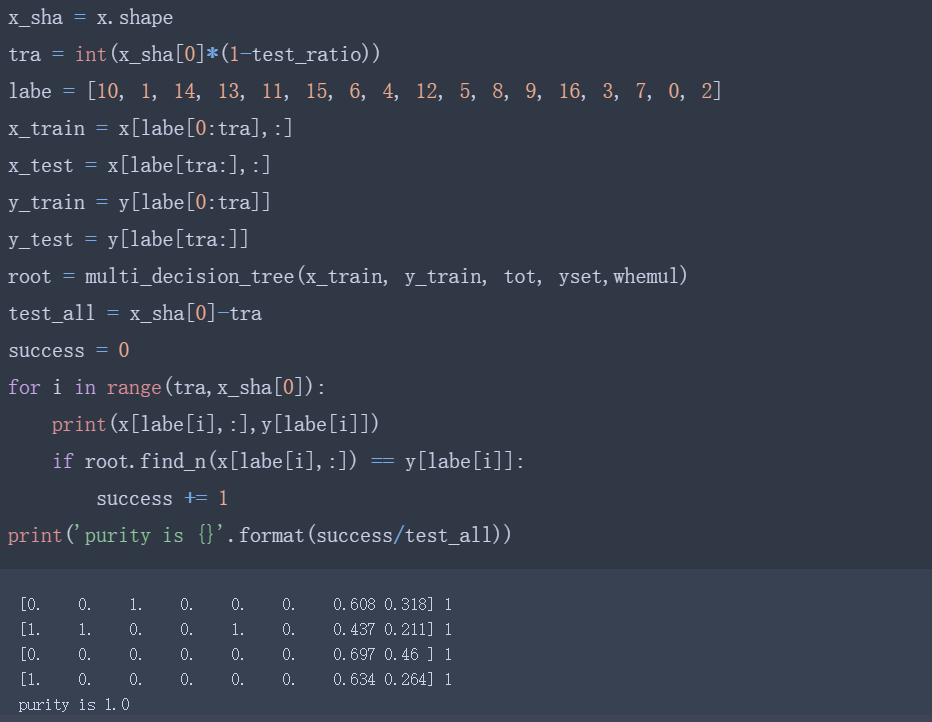
\includegraphics[scale=0.4]{try.PNG}
	\caption{Test}
\end{figure}
附件图(try.png)中给出了学习完毕后,对学习算法的验证(以纯度(impurity)的度量为依据)。

压缩文件中包含了所有的图片和源码。
\end{document}
